\chapter{Monte Carlo Tree Search Agent} \label{chap:MCTS}

The Monte Carlo Tree Search (MCTS) algorithm is a powerful method that has shown great results in games such as chess or Go. The algorithm
works by building a decision tree and using simulations with different strategies to explore the possible outcomes from the current state. 
It iteratively selects and expands the most promising options based on previous simulation results.

The algorithm is divided into four phases: selection, expansion, simulation, and backpropagation. In the selection phase, the algorithm 
traverses the tree from the root to a leaf node, employing a selection strategy, often based on the Upper Confidence Bound (UCB) algorithm, to choose the 
most promising child nodes. Second, the expansion phase adds one or more child nodes to the selected node, representing possible future states 
of the game. Once a leaf node is reached, playouts from the current state are performed until a terminal state is reached. The outcomes of these simulations 
provide feedback about the value of each child node. In the backpropagation phase, these results are used for updating the rewards of each node along 
the path traversed during selection. For a deeper understanding of the algorithm, I recommend reading the paper \cite{winands2017monte} that specifically describes
the application of the MCTS in board games. 

In this section, our focus shifts to the application of Monte Carlo Tree Search in Sagrada. The nodes have the following structure:

\centerline{\mbox{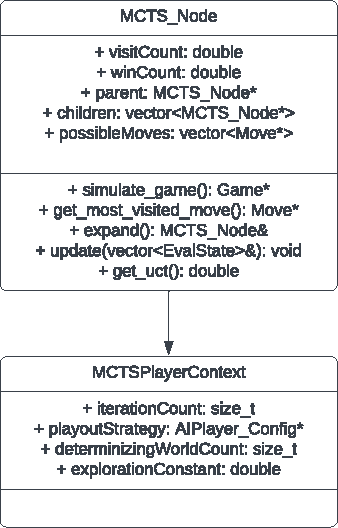
\includegraphics[width=70mm]{img/MCTS_NodeUML.pdf}}}



\section{Selection} \label{sec:MCTS_Selection}

The selection phase in the MCTS algorithm plays a crucial role in efficiently navigating the search tree towards the promising regions while balancing exploration and exploitation. 
One frequently used algorithm for the selection is the Upper Confidence Bound for Trees (UCT) approach being a promising solution for the exploration-exploitation dilemma.

\subsection{Upper Confidence Bound} \label{subsec:MCTS_Selection_UCT}

The UCT formula balances the exploitation of known good actions and the exploration of less explored ones. It calculates the value of each possible action by considering 
both its average reward and the uncertainty associated with it. 

The UCT formula is expressed as:
\[UCT = \bar{X_i} + C \cdot \sqrt{\frac{\ln{N}}{n_i}}\]
where:
\begin{itemize}
    \item $\bar{X_i}$ is the average reward of action i
    \item N is the total number of times the current node has been visited.
    \item ${n_i}$ is the number of times action i has been selected.
    \item $C$ exploration constant balancing exploration and exploitation.
\end{itemize}

Finding an exploration constant that produces the best results possible is not a trivial task. A higher value increases the weight of the exploration term in the formula. 
This leads to more exploratory behavior, as actions that have been sampled less frequently will have a higher UCT value, making them more likely to be chosen.
On the other hand, a lower value of the exploration constant diminishes the influence of the exploration term, thus favoring exploitation. This behavior pushes the 
agent more towards the moves that produced favorable results in the past. A common choice of the exploration factor is $\sqrt{2} $ but in my implementation, I chose
to make the exploration constant a configurable parameter so it was possible to experiment with different constants and compare the results.

The following pseudocode illustrates my implementation of the selection phase:

\begin{algorithm}[H]
    \caption{MCTS Selection}
    \begin{algorithmic}[1]
    \Function{get\_uct}{}
        \State $exploitationFactor \gets winCount / (visitCount \times 5)$
        \State $explorationFactor \gets C \times \sqrt{\frac{\log(parent.visitCount)}{visitCount}}$
        \State \textbf{return} $exploitationFactor + explorationFactor$
    \EndFunction
    
    \Function{select}{$root$}
        \State $currNode \gets root$
        \While{$currNode.is\_fully\_expanded()$ \textbf{and} $!currNode.is\_leaf()$}
            \State $currNode \gets \text{currNode's child that has the highest get\_uct() value}$
        \EndWhile
        \State \textbf{return} $currNode$
    \EndFunction
    \end{algorithmic}
\end{algorithm}


\section{Expansion}

After the selection phase, the expansion step involves adding new nodes to the search tree to explore new parts of the game state space.  If the leaf node is not a terminal state 
and has unexplored actions, the expansion step adds one or more child nodes to the tree corresponding to these actions. Each child node represents a possible action from the current game state.

In my MCTS agent for Sagrada, the moves that lead to new game states represented by the nodes are filtered and sorted using the heuristic filter and the heuristic sort comparator 
described in Sections \ref{sec:Heuristic_filter} and \ref{sec:Heuristic_sort} . For the same reason as in the case of any other agents, these methods are applied to reduce the 
branching factor and to eliminate the weak moves.

\section{Simulation}

The simulation phase, often referred to as playout, is a crucial step in the Monte Carlo Tree Search (MCTS) algorithm where the search tree is traversed from a leaf node to a 
terminal state through a series of simulated gameplays. The primary objective of the simulation phase is to estimate the potential outcome of a game from a given leaf node by 
conducting a series of simulated plays until a terminal state is reached. These simulated plays help in evaluating the quality of the current game state and guide the selection 
of promising actions.

In the simulation phase of the MCTS algorithm, the strategy employed must strike a balance between speed and strength. In my implementation, the playout
strategy of the MCTS player is a configuration parameter that could be changed for different games. This allows experimenting with different strategies to perfect the balance and 
be as strong as possible. Each of the configurable strategies is an AI agent itself such as the Random agent, the Minimax agent or the Rules-based agent.


\section{Backpropagation}

The backpropagation step is responsible for updating the statistics of nodes in the search tree based on the outcome of simulated playouts. This process plays a crucial role in 
guiding the selection towards promising moves. Backpropagation involves updating the statistics of all nodes along the path from the leaf node to the root node. 
The most common technique in backpropagation is to propagate the outcome of the playout (e.g., a win or loss) back up the tree and update the win count and visit count of each node accordingly. 

I decided to use a more sophisticated reward system. The visit count of each node is always incremented by one in the backpropagation phase regardless of the result of the game.
The win count of each node is incremented by 1 if the player wins the game in the simulated playout.  Additional bonuses are awarded based on the player's score differential compared 
to their opponent.  Specifically, the algorithm awards extra points for score differentials of 5, 10, 15, and 20 points. This means that if the player's score is 5 points higher 
than their opponent's, one extra win count is added to the node and it works the same way for the other point t thresholds well. 

This approach ensures that the search tree reflects not only the outcomes of simulated playouts but also considers the significance of score differentials between players pushing
the player towards more promising moves. 

\begin{algorithm}[H]
    \caption{MCTS Backpropagation}
    \begin{algorithmic}[1]
    \Function{update}{$scores$}
        \If{$\text{player that made the move won the simulation}$}
            \State \Call{update\_win\_count}{scores}
        \EndIf
        
        \State $visitCount \gets visitCount + 1$
        \If{$\text{parent exists}$}
            \State \Call{parent.update}{scores}
        \EndIf
    \EndFunction
    
    \Function{update\_win\_count}{$scores$}
        \State $winCount \gets winCount + 1$
        \State $pointThresholds \gets [5,10,15,20]$
        \State $winnerTotalPoints \gets scores[0].get\_total\_points()$
        \State $secondTotalPoints \gets scores[1].get\_total\_points()$
        \For{$pointThreshold$ \textbf{in} $pointThresholds$}
            \If{$winnerTotalPoints - pointThreshold >= secondTotalPoints$}
                \State $winCount \gets winCount + 1$
            \EndIf
        \EndFor
    \EndFunction
    \end{algorithmic}
\end{algorithm}

\section{Handling Imperfect Information}

Leveraging insights from  \cite{long2010understanding}, the MCTS algorithm integrates techniques 
that allow for decision-making under uncertainty. By considering multiple ``possible worlds'', each representing different configurations of opponents' hidden 
objectives and future dice configurations, my MCTS can make more informed decisions. This approach not only adapts the basic MCTS to better handle imperfect 
information but also aligns it with the successful applications of Perfect Information Monte Carlo (PIMC) in other complex games.

% well-known AI textbook by Russell and Norvig 
%   describe properties of games that predict whether PIMC will work well or poorly for any given game

The authors suggest that PIMC search will work well in games that exhibit certain characteristics based on their findings 
from game analyses. These characteristics include:
\begin{itemize}
    \item High Leaf Correlation: Games where the payoffs in terminal nodes (end states) of the game tree are highly correlated, tend to be favorable for PIMC. 
    In these scenarios, the outcome of one decision path often gives a good indication of the outcomes of other, similar paths.
    \item Bias: Games with a high bias, meaning the game inherently favors one player or another in many of its states, also suit PIMC well. In these games, 
    large homogeneous sections of the game tree can be expected, which PIMC can exploit to improve its play efficiency and effectiveness.
    \item Disambiguation Factor: Games where the players' uncertainty about the game state reduces quickly as the game progresses (high disambiguation) 
    are also suitable for PIMC. This factor is significant in games where player actions or game progress naturally narrows down the possible game states or outcomes, 
    allowing PIMC to make more accurate predictions as the game advances.
\end{itemize}

\section{Information Set Monte Carlo}

There are other ways of dealing with imperfect information in the Monte Carlo Tree Search. One of these techniques is called Information Set Monte Carlo.
Information Set Monte Carlo Tree Search (ISMCTS) is an extension of the standard Monte Carlo Tree Search specifically adapted for games with imperfect information, 
here some elements of the game state remain hidden from players. Unlike traditional MCTS, which operates on actual game states, ISMCTS operates on information sets. 
An information set in game theory is a set of possible game states indistinguishable to the player due to the rules of the game masking some information 
(e.g. Private Objective Cards in Sagrada).

Traditional MCTS builds a search tree where each node represents a possible state of the game, and edges represent moves. ISMCTS, however, constructs a tree where nodes 
represent information sets rather than specific states. In games with elements of chance, such as dice selections and rolls in Sagrada, each possible outcome of the dice creates 
a branching path from a node. The other important part of the imperfect information in Sagrada is the Private Objective Card color of the opponent player. 

